\chapter{基于 TLA+ 的 OT函数验证} 
\label{chapter:proof}
\section{TLA+ 简介}
\par TLA+是一种形式化的规约语言。它是一种设计系统和算法的工具,并且用来验证这些系统有没有关键错误。
\par 正确性,是一个系统最为重要的性质,同时,正确性是比较难以证明的,特别是并发系统的正确性,因为存在着数目众多的状态变化。
TLA+可以将系统的行为或者状态抽象为时态逻辑,即系统的行为或者状态会随着时间反生变化,然后通过一些数学分析的方法,来判断系统是否正确。

\par TLA+并不同于一般传统意义上的编程语言,更类似于一种数学语言,因为其语法大部分来自于实际的数理逻辑。
\par TLA+提供了工具集TLAToolbox/TLC,同时还可以使用TLA+的语法糖PLUSCAL来完成代码的编写,由于本文中并未涉及,在此不做展开。
TLA+ model checker 与经典的模型检验工具类似,通过遍历系统模型的所有可能的行为,验证其正确性。

\begin{figure}[H]
\centering
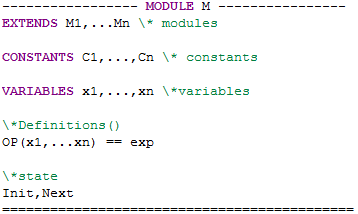
\includegraphics{figures/module.png}
\caption{TLA+编码模板}
\label{fig:graph}
\end{figure}

\subsection{TLA+ Modules}
TLA+ 提供了多种数据结构的实现,包括在本次实验中使用的sequecnce和record等。

record数据结构类似于C语言中的struct结构,即一个record包含若干个field,每个field可以在给定的集合中选取元素填充field。
sequence表示一个序列,如果引入Sequences模块,也可以将数组当作序列来进行处理,并且使用模块里的相应函数
在本次实验中,我们引入了TLA+ 中的Sequences模块,将List表示为一个Sequecnce,并且使用了如下的API:\\
\begin{tabular}{ccc}
\hline
operator& operation& example \\
\hline  
 Head& First element &Head(<<1, 2>>) = 1\\
 Tail& Sequence aside from head &Tail(<<1, 2>>) = <<2>>\\
 Append& Add element to end of sequence &Append(<<1>>, 2) = <<1, 2>>\\ 
 Len& Length of sequence &Len(<<1, 2>>) = 2\\
 $\backslash o$& Connect two sequences &<<1>>\ $\backslash o$\ <<2>> = <<1, 2>>\\
\hline % 
\end{tabular}
\par 以上的操作都不会使原有的操作序列发生变化。

\section{使用 TLA+ 描述 OT 函数}
\subsection{List 相关操作表示}
\subsubsection{第一、二类操作的表示}
采用record的数据结构来表示具体的操作。
第一类操作的record分为两种,set和ins有三个域:pos位置,ch操作字符,pr优先级。而del操作少了ch字符域,这样定义可以减少无效重复的操作数量,使验证代码的效率得到提高。
\begin{align*}
&OP\_1\_set \triangleq [type: \{"set"\}, pos: POS, ch: CH, pr:PR] \\
&OP\_1\_ins \triangleq [type: \{"ins"\}, pos: POS, ch: CH, pr:PR] \\
&OP\_1\_del \triangleq [type: \{"del"\}, pos: POS, pr:PR] \\
&OP\_1 \triangleq OP\_1\_set \cup OP\_1\_ins \cup OP\_1\_del
\end{align*}
第二类操作的record也分为两种,ins操作有三个域:pos插入位置,pr优先级,str要插入的字符串。del操作也有三个域:pos插入位置,pr优先级,len删除区间的长度
\begin{align*}
&OP\_2\_ins \triangleq [type: \{"ins\_r"\}, pos: POS, pr:PR, str:STR] \\
&OP\_2\_del \triangleq [type: \{"del\_r"\}, pos: POS, pr:PR, len:LEN] \\
&OP\_2 \triangleq  OP\_2\_ins \cup OP\_2\_del 
\end{align*}

\subsubsection{第三类操作的表示}
第三类操作同样是使用record来表示,包含两个filed,即type类型和ints删除区间的集合。
\begin{align*}
OP\_3 \triangleq [type:\{"del\_m"\},ints:NoncoSeq] 
\end{align*}

在表示第三类OT函数时,我们首先遇到的问题便是如何表示第三类List命令,由于第三类List命令为删除多个不相交的集合区间,因此我们需要使用TLA+遍历在List长度上所有可以表示出来的区间,一个命令的删除区间即为若干个不相交的符合条件的区间。
在TLA+中支持两个集合的笛卡尔积操作,因此所有符合条件的区间的集合Intervals可以如下定义:
\begin{align*}
Intervals \triangleq \{<a,b> \in POS \times POS: a+b \le Maxnum(POS)+1 \}
\end{align*}
a为区间的起始断点,b为区间长度,因为一个命令的删除区间为若干个不相交的符合条件的区间,定义区间后,便可以生成操作的删除区间。将一个删除操作的删除区间称为一个区间组合,那么有两种方式表示这种区间组合,一种是区间二元组的集合,另一种是二维数组,由于在接下来的OT函数中,需要较为方便地对操作进行转换,所以在本次实验中采用第二种表示方法,先生成第一种表示方法,即二元数组的集合。
\begin{align*}
& NoncoIntervals \triangleq \\ 
& \quad \{ints \in SUBSET \ Intervals : \forall i,j \in ints: i[2]+i[1] \le j[1] \lor j[2]+j[1] \le i[1] \lor i=j\} \backslash \{\{\}\}
\end{align*}
这样,$NoncoIntervals$中每个元素都是一个区间组合,下面我们需要将这个集合变成一个二维数组,由于在TLA+中没有执行某个指令固定次数的相应代码,所以在本次实验中需要多次使用递归来表示这种循环操作。一个符号在使用前必须先声明或者定义,所以使用递归要在函数或定义之前加上recursive关键字。
那么比如在这里我们需要将区间组合的集合转换为区间组合的数组,就需要使用两个递归的定义。
首先定义了将集合转化为序列的SetTOSeq():
\begin{align*}
RECURSIVE\ SetTOSeq(\_)\\
SetTOSeq(T) \triangleq &IF\ T =\ \{\}\ THEN <<>>\\
                       & ELSE\ LET\ t \triangleq CHOOSE\ x \in T : TRUE\\
                        & \quad IN\ <t>\ \backslash o\ SetTOSeq(T \backslash {t})
\end{align*}
接下来便可以定义Seqset(T),将二元组的集合的集合T转化为二维数组的集合:
\begin{align*}
&RECURSIVE\ Seqset(\_)\\
&Seqset(T) \triangleq  \\
& \quad IF\ T = \{\}\ THEN\ \{\}\\
& \quad ELSE\ LET\ t\triangleq\ CHOOSE\ x\ \in T : TRUE\\
& \quad IN\ Seqset(T \backslash {t}) \cup {SetTOSeq(t)} \\
&NoncoSeq\ \triangleq\ Seqset(NoncoIntervals)
\end{align*}
得到的集合$NoncoSeq$便为ints域的取值范围,这样遍历时得到的具体操作的ints域便为一个二维数组,该数组中横坐标表示第几个删除区间,纵坐标1的值表示该区间开始端点,纵坐标为2的值表示区间长度。

\subsection{命令执行的表示}
命令的执行与LIST和具体操作相关,所以定义中使用的参数便是LIST和具体操作中的参数,使用Sequences模块中的API进行代码的编写。
以第二类的del操作为例,调用了 $\backslash o$和$SubSeq$定义:
\begin{align*}
del\_ran\_op(list,pos,len) \triangleq SubSeq(list, 1, pos-1) \quad \backslash o \quad SubSeq(list, pos+len, Len(list))
\end{align*}
唯一不同的是第三类操作的执行函数,同样是由于需要采用循环操作,所以还是要使用递归的定义完成命令的执行。
\begin{align*}
&RECURSIVE\ del\_mulran\_op(\_,\_,\_)\\
&del\_mulran\_op(list,ints,num) \triangleq \\
&  \quad  IF\ num = 0\ THEN\ list \\
&  \quad  ELSE\ del\_mulran\_op(SubSeq(list, 1, ints[num][1]-1)\ \backslash o\ SubSeq(list, ints[num][2]\\
&   \quad \quad  +ints[num[1],Len(list)),ints,num-1)    
\end{align*}
num是ints的区间个数,从后往前进行删除,这样不会影响下面要操作的区间,每次递归删除一个区间,并且值就是删除后的list,当num为0时就表示删除完成了,直接返回当前的参数中的list即可。

\subsection{OT函数的描述}
使用定义Xform表示OT函数,即Xform(lop, rop)为lop对于rop转换后的新操作。
以第一类函数为例:
\begin{align*}
&Xform(lop, rop) \triangleq \\
   & CASE \quad lop.type = "ins" \land rop.type = "ins" -> Xform\_ins\_ins(lop, rop)\\
   & []  \quad lop.type = "ins" \land rop.type = "del" -> Xform\_ins\_del(lop, rop)  \\
   & [] \quad  lop.type = "ins" \land rop.type = "set" -> Xform\_ins\_set(lop, rop)  
\end{align*}
\subsubsection{第一类函数的表示}
第一类函数的表示较为简单,不需要使用递归结构。
以$ins$操作对于$ins$操作的转换来举例说明,使用定义$Xform\_ins\_ins$表示OT函数,即$Xform\_ins\_ins(lins, rins)$为$ins$操作对于$ins$操作转换后的新操作。
\begin{align*}
&Xform\_ins\_ins(lins, rins) \triangleq \\
    &\quad IF \quad lins.pos < rins.pos\\
    &\quad THEN \quad lins\\
    & \quad \quad ELSE \quad IF \quad lins.pos > rins.pos\\
        & \quad \quad \quad THEN \quad [lins \quad EXCEPT !.pos = @ + 1]\\
        & \quad \quad \quad ELSE \quad IF \quad lins.pr < rins.pr\\
                &\quad \quad \quad \quad THEN \quad [lins \quad EXCEPT !.pos = @+1]\\
                &\quad \quad \quad \quad ELSE \quad  lins
\end{align*}
其中EXCEPT !的意思为除了特定的域发生变化,其他域保持不变。
这样参照着之前第一类函数的数学公式,便可以类似地将其他第一类函数用同样的方式表示出来。
\subsubsection{第二类函数的表示}
第二类函数的表示也比较简单,同样不需要使用递归结构。
以$ins$操作对于$del$操作的转换来举例说明,使用定义$Xform\_ins\_del\_r$表示OT函数,即$Xform\_ins\_del\_r(ins, del)$为$ins$操作对于$del$操作转换后的新操作。
\begin{align*}
&Xform\_ins\_del\_r(ins,del) \triangleq \\
   & \quad CASE ins.pos \le del.pos -> ins \\
   & \quad [] ins.pos > del.pos \land ins.pos < del.pos + del.len -> NOP \\
   & \quad [] ins.pos \ge del.pos + del.len -> [ins \quad EXCEPT !.pos = @ - del.len] 
\end{align*}
EXCEPT !的意思为除了特定的域发生变化,其他域保持不变。
这样参照着之前第二类函数的数学公式,便可以类似地将其他第二类函数用同样的方式表示出来。
\subsubsection{第三类函数的表示}
第三类函数为第三类的Del命令与第二类命令中的Ins操作之间的OT函数,以及第三类Del命令自身的OT函数,共2+1=3个。
这类函数的设计代码量占到了整个设计的一半,大量使用了递归定义,这里拿最为复杂的Del命令自身的OT函数来举例。
\begin{align*}
&RECURSIVE\ Xform\_del\_del\_m(\_,\_,\_)\\
&Xform\_del\_del\_m (ldel,rdel,i) \triangleq \\
& \quad IF\ i > Len(ldel.ints)\ THEN\ ldel\\
& \quad \quad  ELSE\ Xform\_del\_del\_m ([ldel\ EXCEPT !.ints[i]= transdel4(@,rdel.ints)],rdel,i+1)
\end{align*}
使用定义$Xform\_del\_del\_m$表示OT函数,这里设置i为递归变量,i为ldel中当前正在进行转换的区间,转换函数为transdel4,按照公式(3-10)进行编写,即进行一个删除区间相对于rdel的转换,这样当i的值大于ldel中删除区间的数量时,所有删除区间都完成了转换,将转换后的新区间合并起来,便是ldel转换后的新操作。
\begin{align*}
&transdel4(int,ints) \triangleq \\ 
  & \quad <<newpos(int[1],ints,1),newlen(int[1],int[2],ints,1,0)   >>
\end{align*}
$newpos$和$newlen$便是这个删除区间对于rdel的转换后的新区间端点和区间长度。
$newpos$和$newlen$两个定义同样使用递归结构来表示。
$newpos$:
\begin{align*}
& RECURSIVE newpos(\_,\_,\_)\\
& snewpos(pos,ints,i) \triangleq\\
&\quad IF \ pos < ints[1][1] \ THEN \ pos\\
&\quad ELSE \ IF \ i=Len(ints) \land pos \ge ints[i][1] + ints[i][2] \ THEN \ pos - Dlen(ints,i,0)\\
&\quad ELSE \ IF \ pos \ge ints[i][1] \land pos < ints[i][1] + ints[i][2] \ THEN \ ints[i][1] - Dlen(ints,i-1,0)\\
&\quad ELSE \ IF \ ints[i][1] + ints[i][2] \le pos \land pos < ints[i+1][1] \ THEN \ pos - Dlen(ints,i,0)\\
&\quad ELSE \ newpos(pos,ints,i+1)
\end{align*}
递归变量为i,代表当前在对rdel中第几个区间进行newpos的计算,每递归一次,i的值加一,如果满足条件要求则返回相应newpos的值。其中Dlen的作用为统计rdel中前i个删除区间的长度之和。
$newlen$:
\begin{align*}  
&RECURSIVE newlen(\_,\_,\_,\_,\_)     \\
&newlen(pos,len,ints,i,sum) \triangleq\\
    & \quad IF\ i > Len(ints) \ THEN \quad len - sum\\
    & \quad ELSE \ IF \ pos + len < ints[i][1] \ THEN \ newlen(pos,len,ints,i+1,sum)\\
    & \quad ELSE \ IF \ pos < ints[i][1] \land ints[i][1] < pos + len \land pos + len \le ints[i][1] + ints[i][2]\\
    & \quad \quad THEN \ newlen(pos,len,ints,i+1,sum + pos + len -ints[i][1])\\
    & \quad ELSE \ IF \ pos < ints[i][1] \land pos + len > ints[i][1] + ints[i][2]\\
    & \quad \quad THEN \ newlen(pos,len,ints,i+1,sum + ints[i][2])\\
    & \quad ELSE \ IF \ ints[i][1] \le pos \land pos < ints[i][1] + ints[i][2] \land pos + len \le ints[i][1] + ints[i][2]\\
    & \quad THEN \ 0\\
    & \quad ELSE \ IF\ ints[i][1] \le pos \land pos < ints[i][1] + ints[i][2] \land pos + len > ints[i][1] + ints[i][2] \\
    & \quad \quad THEN \ newlen(pos,len,ints,i+1,sum + ints[i][1] + ints[i][2] - pos)    \\
    & \quad ELSE \ newlen(pos,len,ints,i+1,sum)
\end{align*}
递归变量为i和sum,i表示当前在对rdel中第几个区间进行newlen的计算,sum表示在当前计算完成的所有区间中len转换为newlen需要减去的长度。
这样便根据公式(3-10)完成了Del命令自身的OT函数,第三类的Del命令与第二类命令中的Ins操作之间的OT函数可以用类似地方式表示出来。
同时,剩余的OT函数也可以用递归或非递归的形式根据公式进行表示,在此不再赘述。
\section{正确性验证}
上节中已经完成了OT函数的TLA+描述,剩下的就是决定验证的目标和方式。

我们验证CP1性质的正确性。即同一个List经过OT(OP2,OP1),OP1或者OT(OP1,OP2),OP1这两种操作序列后,最终的结果应该是一致的。
结合以上给出的定义,用TLA+来描述所设计OT函数的CP1正确性:
\begin{align*}
  apply(apply(list,op1),Xform(op2, op1)) = apply(apply(list,op2),Xform(op1, op2))
\end{align*}
\par 只要对于任意的两个操作,这个等式都成立的话,那么CP1正确性即可得到验证。

因为在本次实验中不涉及系统状态的变化,只需证明等式对于所有操作都成立即可,因此没有behavior spec,即没有初始状态 Init 和状态关系 Next。不过,在TLC中提供了Evaluate Constant Expression的功能,即可以计算常量表达式的值。以第一类函数的CP1验证为例,我们给出如下正确性定义:
\begin{align*}
 & correctness_1 (list) \triangleq \\
 & \quad \forall op1,op2 \in OP_1:\\
 & \quad \quad \lor op1.pr = op2.pr\\
 & \quad \quad \lor apply(apply(list,op1),Xform(op2, op1)) = apply(apply(list,op2),Xform(op1, op2))  
\end{align*}
这样的话,$op1$,$op2$就实现了对$OP_1$中所有操作的遍历,并且对于满足要求的任意$op1$和$op2$,只要优先级满足要求(两个操作的优先级不相等),则其一定满足CP1等式。
在Evaluate Constant Expression内填写这个表达式,我们便可以check model并根据value的值来检验函数的正确性了。

\subsection{TLA+ Model Checker 设置及实验环境}
在本次实验中,我们定义Model Checker中常量的参数值如下:\\
STR <- \{"like","enjoy","fond","love","fantasy"\} \\
CH <- \{"a","b","c","d","e"\}\\
PR <- \{1,2\}\\
STR为第二类插入操作中str域的可选择范围,CH为第二类插入、设置操作中ch域的可选择范围,PR为操作的优先级,在此处我们设定两个操作的优先级不相同,否则为违规操作变换。
通过调整LIST常量的长度,实验在不同长度的LIST下完成各类函数的验证所需要的时间。\\

实验环境:\\
Number of worker threads: 12\\
Fraction of physical memory allocated to TLC: 16173 mb

\subsection{实验结果}
\begin{figure}[H]
\centering
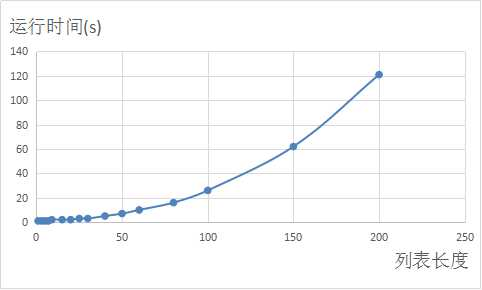
\includegraphics{figures/runtime1.bmp}
\caption{验证第一类函数正确性的运行时间与列表长度(横坐标)的关系}
\end{figure}
\par 结果分析:若列表长度为n,则第一类操作的个数:$5*2*n(ins)+5*2*n(set)+2*n(del) = 22n$。
任意选取其中两个操作验证CP1正确性,所以验证算法的时间复杂度为$O(n^2)$。
从实验结果看,与复杂度的分析相一致。

\begin{figure}[H]
\centering
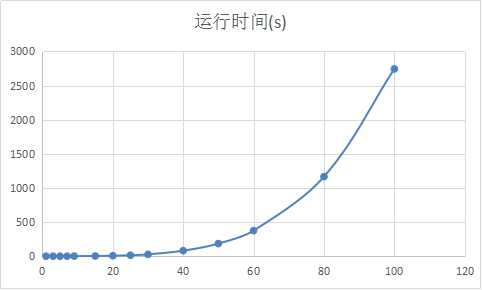
\includegraphics{figures/runtime2.bmp}
\caption{验证第二类函数正确性的运行时间与列表长度(横坐标)的关系}
\end{figure}
\par 结果分析:若列表长度为n,则第二类操作的个数:$5*2*n(ins))+n*2*n(del) = 2n^2+10n$。
任意选取其中两个操作验证CP1正确性,所以验证算法的时间复杂度为$O(n^4)$。
从实验结果看,与复杂度的分析相一致。

\begin{figure}[H]
\centering
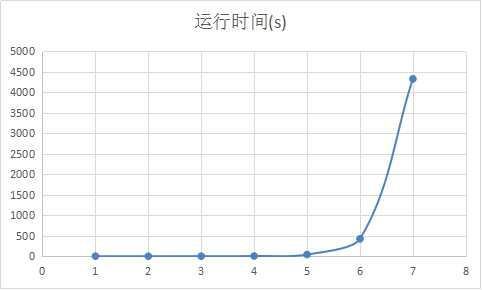
\includegraphics{figures/runtime3.bmp}
\caption{验证第三类函数正确性的运行时间与列表长度(横坐标)的关系}
\end{figure}
\par 结果分析:目前第三类函数的验证结果只能到LIST长度为7。
因为第三类操作的个数为指数级别$O(3^n)$,并且在生成操作和操作的转换过程中多次使用了递归,更大大增加了验证算法的复杂程度。

\begin{figure}[H]
\centering
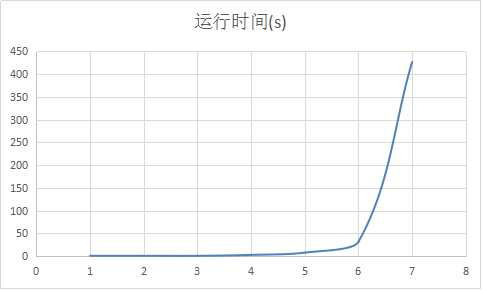
\includegraphics{figures/runtime4.bmp}
\caption{验证其余函数正确性的运行时间与列表长度(横坐标)的关系}
\end{figure}
\par 结果分析:目前其余函数的验证结果只能到LIST长度为7。
与第三类函数的验证相同,在其余函数的验证算法中也需要生成$O(3^n)$级别的第三类操作和使用递归代码实现操作的转换,因此复杂度与第三类函数相仿。

\begin{figure}[H]
\centering
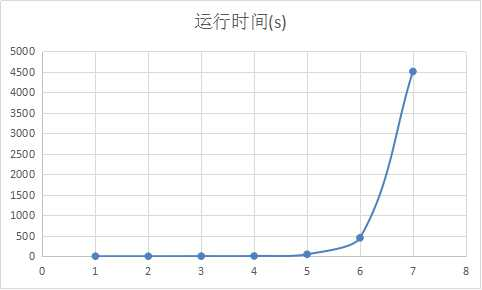
\includegraphics{figures/runtimeall.bmp}
\caption{验证所有OT函数正确性与列表长度(横坐标)的关系}
\end{figure}
\par 结果分析:时间复杂度与第三类函数的复杂度相同,目前可以验证所设计的OT函数在LIST长度为7之内时的正确性。

经过TLA+的验证,大大提高了我们所设计函数的可信度。